% Expos� � COIMBRA, 10 mars 2007
%

\documentclass[%
pdf,        %for a pdf file  (other: ps)
%ps,
nocolorBG,  %white background (other: colorBG)
%colorBG,
nototal,    % only the number of slide (other: total)
%total,
slideColor, % slides will use many colors
%slideBW,
final,      % final mode (other: draft)
%draft,
%frames  %fond blanc graphes OK
%azure
sophie % graphiques bnon
%nuancegris %graphiques tiennent pas
%troispoints %fond noir
%lignesbleues %fond noir
%darkblue titre coupes, graphiques tiennent pas
%alienglow fond noir
%autumn
]{prosper}

\usepackage[latin1]{inputenc}
\usepackage{amsmath} 
\usepackage{a4wide}
\usepackage{pstricks,pst-node,pst-text,pst-3d}
\usepackage{multicol}
\usepackage{graphicx,graphics}
\usepackage{color}
\usepackage{lscape}
\usepackage{array}
\usepackage{epsfig}


\newcommand{\Acal}{\mathcal{A}}
\newcommand{\m}{\mathbf{m}}
\newcommand{\esp}{\mathbb{E}}
\newcommand{\pr}{\mathbb{P}}
\newcommand{\prob}{\mathbb{P}}
\newcommand{\eps}{\epsilon}
\newcommand{\Imoins}[2]{I_{#1}(#2)}
\newcommand{\ind}{1 \hspace{-1.2mm} \mbox{I}}
\newcommand{\Esp}{\mathbb{E}}
\newcommand{\Vsf}{\mathsf{V}}
\newcommand{\Xbf}{{\bf X}}
\newcommand{\autm}{\mbox{aut}(\mathbf{m})}
\newcommand{\Omegas}{\underset{s}{\Omega}}
\newcommand{\mbf}{{\bf m}}
\newcommand{\mum}{\mu(\mathbf{m})}
\newcommand{\Ncal}{\mathcal{N}}
\newcommand{\Obf}{{\bf 0}}
\newcommand{\Pcal}{\mathcal{P}}
\newcommand{\Rcal}{\mathcal{R}}
\newcommand{\Var}{\mathbb{V}\text{ar}}
\newcommand{\Lcal}{\mathcal{L}}
\newcommand{\Zbf}{{\bf Z}}


\definecolor{orange}{rgb}{.98,.51,.03}
\definecolor{vert}{rgb}{0.09,0.7,0.17}
\definecolor{violet}{rgb}{0.69,0.13,0.69}

\newcommand{\orangebullet}{\textcolor{orange}{{\footnotesize$\bullet$}}}
\newcommand{\bluebullet}{\textcolor{blue}{{\footnotesize$\bullet$}}}
\newcommand{\itemorange}{\item[\orangebullet]}
\newcommand{\itemblue}{\item[\bluebullet]}
\newcommand{\org}[1]{\bfseries\textcolor{orange}{#1}}
\newcommand{\rose}[1]{\bfseries\textcolor{magenta}{#1}}

%=================================================

\title{\textcolor{blue}{Assessing the exceptionality of \\network motifs}}
\author{F. Picard, J.-J. Daudin, \underline{S. Schbath},
        S. Robin}
\institution{\textcolor{orange}{\textbf{S}}tatistics for \textcolor{orange}{\textbf{S}}ystems \textcolor{orange}{\textbf{B}}iology, Jouy-en-Josas/Evry/Paris, France
              

\vspace{1mm}

\textcolor{orange}{\bfseries \url{http://genome.jouy.inra.fr/ssb/}}

\vspace{4mm}

Acknowledgments: E. Birmel�, C. Matias

\vspace{5mm}


\includegraphics[width=3cm]{/home/mig/schbath/Images/INRA/LogoINRA-Couleur.eps}\hfill
\includegraphics[width=3cm]{/home/mig/schbath/Images/INRA/mig_7_small.ps}
%\includegraphics[width=3cm]{/home0/mig/schbath/Images/INRA/logoinra.ps}\hfill
%\includegraphics[width=3cm]{/home0/mig/schbath/Images/INRA/mig_7_small.ps}
}
\slideCaption{WSGP follow up meeting, Coimbra, March 9-10, 2007}


\begin{document}

\maketitle


%----------------------------------------------------
\overlays{1}{%
\begin{slide}{The network revolution}

\parbox{6cm}{
\begin{itemize}
\itemorange \textbf{Many scientific fields}: \\
 sociology, physics, "internet", biology.

 \itemorange \textbf{Nature of the data}:\\
 -- interactions between $n$ elements,\\
 -- $n^2$ possible interactions.

\itemorange \textbf{Topology of the network:} \\
-- describes the way genes/proteins interact,\\
-- structural properties (degrees, diameter, clustering coefficient).
\end{itemize}
}
\parbox{5cm}{

\vspace{-10mm}
\begin{center}
\includegraphics[angle=90,height=6cm,width=6cm]{./figures/barabasi6.ps}\\
\begin{tiny} \qquad\qquad From Barabasi et al.(2004) \end{tiny}
\end{center}
}

\end{slide}
}
%----------------------------------------------------


%----------------------------------------------------
\overlays{1}{%
\begin{slide}{Looking for local structures in biological networks}

\begin{itemize}
\itemorange \textbf{Breaking-down complex networks into functional
  modules or basic building blocks}: 
\textcolor{violet}{\scriptsize[Shen-Orr et al. (02)]}\\
 {\bf{$\rightarrow$}} patterns of interconnection,
  \textbf{\textcolor{orange}{motifs}}.

 \vspace{-5mm}

\itemorange \textbf{Transcription regulatory networks}:
\hfill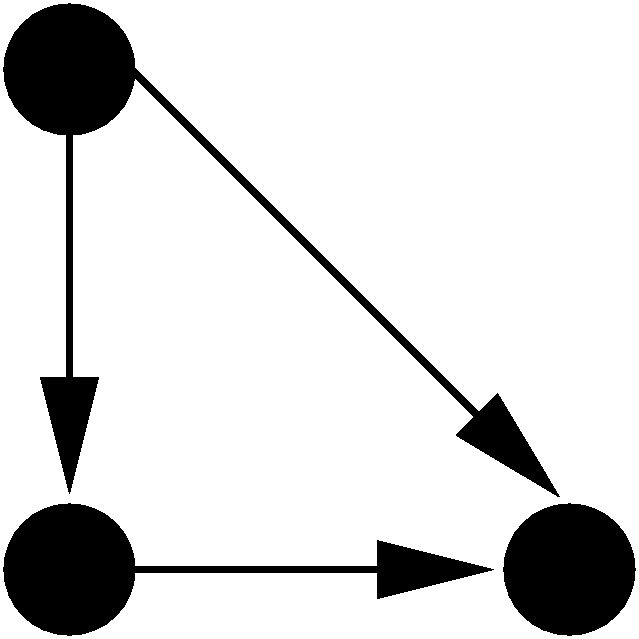
\includegraphics[width=1cm]{./figures/feedforwardloop.eps}\\
 motifs may perform specific regulatory functions\\
 (e.g. feed-forward loop, bi-fan).
 \vspace{-5mm}

\itemorange \textbf{Focus on exceptional motif} 
\hfill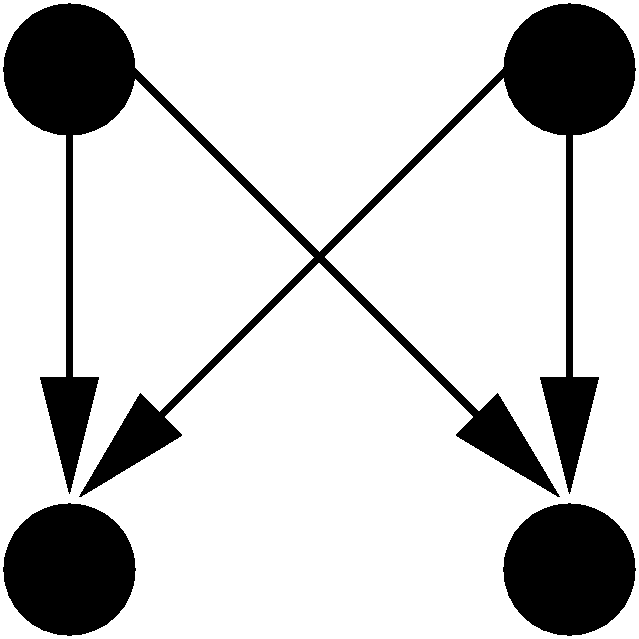
\includegraphics[width=1cm]{./figures/bifan.eps}\\
 $=$ motifs appearing more frequently than
 \textbf{expected}. \\
\textcolor{violet}{\scriptsize[Milo et al. (02), Shen-Orr et al. (02), Zhang
  et al. (05)]}\\
\itemorange \textbf{Interpretation}: \\
\bluebullet\ they are thought to reflect functional units which combine to regulate
the cellular behavior as a whole,\\
\bluebullet\ mathematical analysis of their dynamics are required.
\textcolor{violet}{\scriptsize[Mangan and Alon (03), Prill et al. (05)]}


\end{itemize}

\end{slide}
}
%----------------------------------------------------


%----------------------------------------------------
\overlays{1}{%
\begin{slide}{How to assess the exceptionality of a motif?}

\begin{description}
\item[\org{Step 1}] \textbf{Counting} the observed number $N_{\text{obs}}(\mbf)$ of a
  given motif $\mbf$ (out of our scope)
\end{description}
Its significance is assessed with the $p$-value
{\scriptsize$\mathbb{P}\{N(\mbf) \geq N_{\text{obs}}(\mbf)\}$}
\begin{description}
\item[\org{Step 2}] Choosing an appropriate \textbf{random graph model} 
\item[\org{Step 3}] Getting the \textbf{distribution} of the count $N(\mbf)$
\end{description}
\begin{itemize}
\itemblue Asymptotic approximations (Poisson, Gaussian) exist under some very restrictive hypothesis. 
\itemblue For now, the  $p$-value is obtained thanks to simulations:
\\
-- random networks generated by edge swapping,\\
-- empirical distribution ($\rightarrow$ heavy simulations),\\
-- or using a $Z$-score ($\rightarrow$ Gaussian approximation).
\end{itemize}

\end{slide}
}
%----------------------------------------------------

%----------------------------------------------------
\overlays{1}{%
\begin{slide}{Our contribution}

\begin{itemize}
\itemorange To provide analytical expressions of the mean and the variance
of the count  in a wide class of random graph models.
\itemorange To propose a relevant distribution to approximate the count
distribution.

\itemblue To propose a new random graph model adapted for biological networks.
\end{itemize}
\end{slide}
}
%----------------------------------------------------

%----------------------------------------------------
\overlays{1}{%
\begin{slide}{Random graphs}

\begin{itemize}
\itemorange A random graph is defined by: \\
\begin{itemize}
\itemblue a set $\mathcal{V}$ of fixed vertices with $|\mathcal{V}|=
n$,
\itemblue a set of random edges $\Xbf=\{ X_{ij}, (i,j) \in
\mathcal{V}^2\}$   such that 
$$
X_{ij}=\left\{\begin{array}{ll}
1& \text{if } i \text{ and } j \text{ are connected},\\
0& \text{otherwise}
\end{array}\right.
$$

\itemblue and a distribution on $X_{ij}$. 
\end{itemize}

\itemorange Examples: 
\begin{itemize}
\itemblue the Erd\"os-R�nyi model,

\itemblue the ERMG model.
\end{itemize}
\end{itemize}
\end{slide}
}
%----------------------------------------------------

%----------------------------------------------------
\overlays{1}{%
\begin{slide}{Example: Erd�s-R�nyi model}

\begin{itemize}
\itemorange Edges $X_{ij}$'s are independent $\ldots$

\itemorange $\ldots$ and identically distributed according to $\mathcal{B}(\pi)$
$$
\mathbb{P}(X_{ij}=1)=\pi
$$

\itemorange Degrees are Poisson distributed

$$
K_i:=\sum_{j\neq i} X_{ij}\sim \mathcal{B}(n-1,\pi)\approx \mathcal{P}((n-1)\pi)
$$

\itemblue It does not fit with biological networks. \\
The main reason is: heterogeneity.\\
\quad

\itemblue Our first alternative was
$\mathbb{P}(X_{ij}=1)\propto d_id_j$\\
\textcolor{violet}{\scriptsize[Matias, Schbath, Birmel�, Daudin and Robin (06)]}

\end{itemize}
\end{slide}
}
%----------------------------------------------------

%----------------------------------------------------
\overlays{1}{%
\begin{slide}{Example: Erd�s-R�nyi Mixture for Graphs}

\begin{itemize}
\itemorange Vertices are spread into $Q$ groups.

\itemorange Conditionally to the group of vertices, edges are
independent and
$$
X_{ij}\:|\:\{i\in q, j\in \ell\} \sim \mathcal{B}(\pi_{q,\ell})
$$
$\pi_{q,\ell}$ is the connection probability between
groups $q$ and $\ell$.

\itemorange Degrees are distributed according to a Poisson mixture

$$
K_i\sim \sum_q \alpha_q \mathcal{B}(n-1,\overline{\pi}_q) 
\text{ with }
\overline{\pi}_q=\sum_{\ell}\alpha_{\ell} \pi_{q,\ell}
$$

\itemblue Better fit to biological networks.

\end{itemize}

\centerline{\textcolor{violet}{\scriptsize[Daudin, Picard and Robin (07)]}}
\end{slide}
}
%----------------------------------------------------

%----------------------------------------------------
\overlays{1}{%
\begin{slide}{ERMG flexibility}

\begin{tabular}{m{3cm}m{2cm}cc}
Examples & Network & $Q$ & $\pi$ \\\hline
Erd�s-R�nyi
& \includegraphics[angle=90,height=1.5cm]{./figures/FigNetworks-Erdos-Col.eps}
& 1 & $p$\\\hline
Independent model (product connectivity)
& \includegraphics[angle=90,height=1.5cm]{./figures/FigNetworks-Indep-Col.eps}
& 2 & $\left(\begin{array}{cc}a^2 & ab\\ ab&b^2\end{array}\right)$\\\hline
Stars
&
\includegraphics[angle=90,height=1.5cm]{./figures/FigNetworks-Star-col.eps}
& 4 & {\renewcommand{\arraystretch}{0.3}\scriptsize$\left(\begin{array}{cccc}0&1&0&0\\
                                1&0&1&0\\
                                 0&1&0&1\\
                                 0&0&1&0\end{array}\right)$}\\\hline
Clusters (affiliation network)
&\includegraphics[angle=90,height=1.5cm]{./figures/FigNetworks-Clusters-Col.eps}
& 2 & $\left(\begin{array}{cc}1& \varepsilon\\ 
                               \varepsilon&1\end{array}\right)$\\
\end{tabular}



\end{slide}
}
%----------------------------------------------------

%----------------------------------------------------
\overlays{1}{%
\begin{slide}{Network motifs}

\begin{itemize}
 \itemorange Let $\mbf$ be a motif of size $k$ {\scriptsize (connected sub-graph
 with $k$ vertices)}.

\itemorange Definition through its adjacency
matrix (also denoted by $\mbf$) such that $\mbf_{uv}=1$, if nodes $u$
and $v$ are connected in the motif and 0 otherwise.

\itemorange Ex: 3 versions of the $\mathsf{V}$ motif at a \textbf{fixed} position $(i,j,k)$.
\end{itemize}
\begin{center}
\tiny
\begin{tabular}{|ccc|}
\hline
$\mbf$ &  $\mbf^{\prime}$ & $\mbf^{\prime \prime}$ \\
\hline
\hline
& & \\
$\left[ \begin{array}{ccc} 0 & 1 & 1 \\ . & 0 & 0 \\ . & . & 0 \end{array} \right]$  &
$\left[ \begin{array}{ccc} 0 & 1 & 0 \\ . & 0 & 1 \\ . & . & 0 \end{array} \right]$ &
$\left[ \begin{array}{ccc} 0 & 0 & 1 \\ . & 0 & 1 \\ . & . & 0 \end{array} \right] $ \\
&&
\\
\includegraphics[angle=0,height=15mm]{./figures/version2.eps} & 
\includegraphics[angle=0,height=15mm]{./figures/version3.eps} & 
\includegraphics[angle=0,height=15mm]{./figures/version1.eps} \\
\hline
\end{tabular}
\vspace{-0.2cm}
\end{center}

\end{slide}
}
%----------------------------------------------------
%\end{document}

%----------------------------------------------------
\overlays{1}{%
\begin{slide}{Position and occurrence of a motif}

\begin{itemize}
\itemorange Let $\alpha$ be a possible position of $\mbf$. We consider that $\alpha$ is an ordered $k-$tuple $(i_1,\ldots,i_k)$
with $i_1<\hdots<i_k$. 

\itemorange Let $Y_{\alpha}(\mbf)$ be the random indicator
variable  such that
$$
Y_{\alpha}(\mbf)=\left\{\begin{array}{ll}
1& \text{if } \mbf \text{ occurs at position } \alpha,\\
0& \text{otherwise}
\end{array}\right.
$$
Formally we have
$$
Y_{\alpha}(\mbf) = \prod_{1 \leq u < v \leq k}
\left(\textcolor{red}{X_{i_u i_v}}\right)^{\textcolor{black}{m_{uv}}}.
$$
\end{itemize}
\end{slide}
}
%----------------------------------------------------


% %----------------------------------------------------
% \overlays{1}{%
% \begin{slide}{Motif permutation}

% \vspace{-1cm} 
%  \begin{itemize}
%  \item[$\blacktriangleright$]Let $\mathfrak{S}$ be the set of permutations on the vertices of $\mbf$. We need to consider 
% \begin{equation*}\autm = \{\sigma \in \mathfrak{S},\; \sigma(\mbf) = \mbf \}\end{equation*}
%  \item[$\blacktriangleright$] Then we define $\mathcal{R}(\mbf)$, the set of non redundant permutations of $\mbf$, and we denote 
% \begin{equation*}\rho(\mbf)=|\mathcal{R}(\mbf)|=k!/|\autm|\end{equation*}
%  \item[$\blacktriangleright$] We consider \textbf{permutations of the motif} rather than permutations of positions.
%   \item[$\blacktriangleright$]We consider the $k!$ simultaneous permutations of the rows and columns of $\mbf$.
%  \end{itemize}
% \begin{center}
% \begin{tabular}{cc}
% \begin{tabular}{c}
% $\text{aut}(\mathsf{V}) = \left\{\text{Id}, (2,3) \right\}$ \\
% \includegraphics[angle=-90]{./figures/Vaut.eps} 
% \end{tabular}
% & 
% \begin{tabular}{c|cccc}
%  & 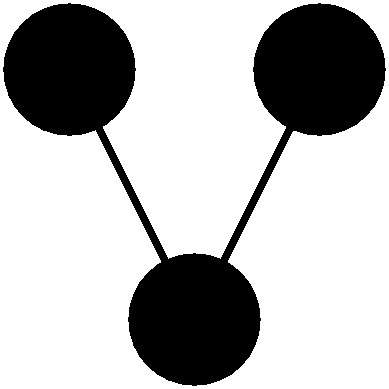
\includegraphics{./figures/Vmotif.eps} & 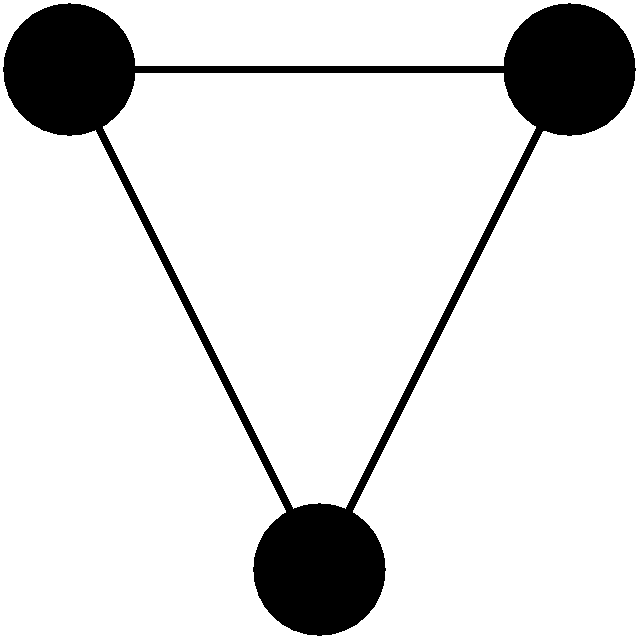
\includegraphics{./figures/nablamotif.eps} & 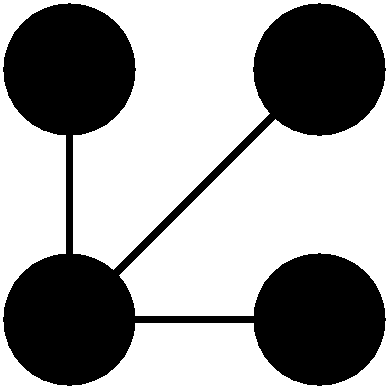
\includegraphics{./figures/starmotif.eps}  & 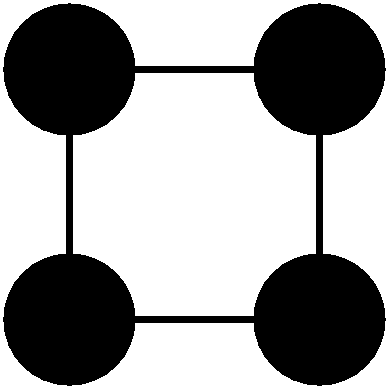
\includegraphics{./figures/squaremotif.eps}\\
%  \hline
%  $|\autm|$ & 2 & 6 & 6 & 8\\
%  $\rho(\mbf)$ & 3 & 1 & 4 & 3\\
%  \end{tabular} 
% \end{tabular}
 
% \end{center}
% \end{slide}
% }
% %----------------------------------------------------

%----------------------------------------------------
\overlays{1}{%
\begin{slide}{Number of occurrences of a motif}

\begin{itemize}
\itemorange Let $\mathcal{R}(\mbf)$ be the set of non redundant
permutations of $\mbf$ (so-called ``versions''),

\itemorange and $I_k$ the set of ordered $k$-tuples from $\mathcal{V}$ ($|I_k|=\binom{n}{k}$).
\end{itemize}

\vspace{5mm}

\begin{itemize}
\itemblue The count $N(\mbf)$ of motif $\mbf$ is then:
 $$
 N(\mbf) =  \sum_{\alpha \in I_k} \sum_{\mbf^\prime \in \mathcal{R}(\mbf)} Y_{\alpha}(\mbf^{\prime}).
 $$
$\Rightarrow$ We consider \textbf{permutations of the motif}
rather than permutations of positions. 

  \end{itemize}
\end{slide}
}
%----------------------------------------------------

%----------------------------------------------------
\overlays{1}{%
\begin{slide}{Model assumptions}

\begin{itemize}
\itemorange \textcolor{orange}{\textbf{stationarity}}: 
$\mathcal{D}(X_{i_1j_1}, \ldots, X_{i_{\ell}j_{\ell})}=
\mathcal{D}(X_{i'_1j'_1}, \ldots, X_{i'_{\ell}j'_{\ell}})$ .

\vspace{5mm}

$\Rightarrow$ the distribution of
$Y_{\alpha}$ does not depend on $\alpha$.

\vspace{5mm}

Denoting by $\mum$ the
\textbf{occurrence probability} of motif $\mbf$, we have 
$$
Y_{\alpha}(\mbf) \sim \mathcal{B}(\mum)
$$



\itemorange \textcolor{orange}{\bfseries Independence of disjoint occurrences}:
$$
Y_\alpha(\mbf) \perp Y_\beta(\mbf)
\quad \text{ if } \quad \alpha \cap \beta =\emptyset.
$$ 

\itemorange 

  \end{itemize}
\end{slide}
}
%----------------------------------------------------


%----------------------------------------------------
\overlays{1}{%
\begin{slide}{Mean number of occurrences of a motif}

Since 
$$
N(\mbf) =  \sum_{\alpha \in I_k} \sum_{\mbf^\prime \in
  \mathcal{R}(\mbf)} Y_{\alpha}(\mbf^{\prime})
$$
and 
$$
Y_{\alpha}(\mbf') \sim \mathcal{B}(\mum), \quad \forall \mbf^\prime \in
  \mathcal{R}(\mbf),
$$

we have:

$$
\textcolor{blue}{\Esp N(\mbf)} \quad = \quad 
|I_k| \times \sum_{\mbf^\prime \in \mathcal{R}(\mbf)} \Esp
Y_{\alpha}(\mbf^\prime) \quad = \quad 
\textcolor{blue}{\binom{n}{k} |\mathcal{R}(\mbf)| \mum}.
$$

\end{slide}
}
%----------------------------------------------------


%----------------------------------------------------
\overlays{1}{%
\begin{slide}{Variance of the count}

$$
\mathbb{V}\text{ar} N(\mbf) = \Esp N^2(\mbf) - (\Esp N(\mbf))^2 
$$
 
\begin{itemize}
\itemorange Decomposition of $N^2(\mbf)$:
\begin{eqnarray*}
N^2(\mbf) &=&\sum_{\alpha, \beta \in I_k}
\sum_{\mbf^\prime, \mbf^{\prime \prime}\in \mathcal{R}(\mbf)}
Y_{\alpha}(\mbf^{\prime})Y_{\beta}(\mbf^{\prime \prime}),\\
&=& \sum_{s=0}^k \sum_{|\alpha \cap \beta| = s}
\sum_{\mbf', \mbf'' \in \Rcal(\mbf)} Y_{\alpha \cup \beta}(\mbf'
\Omegas \mbf''),
\end{eqnarray*}
\itemorange
where the \textcolor{orange}{\textbf{super-motif}} $\mbf' \Omegas \mbf''$ is the union of
two overlapping occurrences of $\mbf'$ and $\mbf''$.  

\vspace{5mm}

$\Omegas$ is the overlapping operation with $s$ common
vertices.
\end{itemize}

\end{slide}
}
%----------------------------------------------------


%----------------------------------------------------
\overlays{1}{%
\begin{slide}{Super-motifs}

\begin{itemize}
\itemorange Example for the $\mathsf{V}$ motif:
\begin{center}
\includegraphics[height=2cm]{./figures/supermotif.eps}
\end{center}
\begin{itemize}
 \itemblue$\mbf$ occurs at $\alpha=(1,3,4)$, $\mbf'$ occurs at
 $\beta=(2,3,4)$,  

 \itemblue in this case $\alpha \cap \beta = (3,4)$ and $s=2$.
\end{itemize}

\vspace{5mm}

\itemorange The adjacency matrix of the super-motifs $\mbf' \Omegas
\mbf''$ can be  easily derived from the adjacency matrices of $\mbf'$
and $\mbf''$ \textcolor{violet}{\scriptsize[Picard et al. (07)]}.
\end{itemize}
\end{slide}
}
%----------------------------------------------------


%----------------------------------------------------
\overlays{1}{%
\begin{slide}{Variance of the count (end)}

\begin{itemize}
 \itemorange The expectation of $N^2(\mbf)$ is then
$$
\Esp N^2(\mbf)= \sum_{s=0}^k \sum_{|\alpha \cap \beta| = s}
\sum_{\mbf', \mbf'' \in \Rcal(\mbf)} \mu(\mbf'\Omegas \mbf'').
$$
  
\itemorange The independence assumption for $s=0$ gives
$\mu(\mbf'\Omegas \mbf'')=\mu(\mbf)^2$, leading to:
\begin{eqnarray*}
\Esp N^2(\mbf) & = & C_1(n,k) |\Rcal(\mbf)|^2 \mu(\mbf)^2 \\
&&\quad  +  \sum_{s=1}^{k} C_2(n,k,s) \sum_{\mbf', \mbf'' \in \Rcal(\mbf)}
  \mu(\mbf'\Omegas \mbf'').
\end{eqnarray*}

 \itemorange The final point is now the calculation of the occurrence
 probabilities $\mu(\cdot)$.
\end{itemize}
\end{slide}
}
%----------------------------------------------------


%----------------------------------------------------
\overlays{1}{%
\begin{slide}{Calculating $\mum$}

\begin{itemize}
 \itemorange The probability of occurrence of a given motif depends on
 the distribution of the $X_{ij}$'s.

 \itemorange Stationary assumption: $\mum$ does not depend on the
 position of the motif

 \itemblue In the Erd\"os-R�nyi model: $\mum = \pi^{v(\mbf)}$,
 with $v(\mbf)$ the number of edges in $\mbf$.

 \itemblue In the \textbf{ERMG} model with $Q$ groups
   with proportion $\alpha_1,\hdots, \alpha_Q$:
$$
\mum   =   \sum_{c_1=1}^{Q} \hdots \sum_{c_k=1}^{Q}
\alpha_{c_1}\hdots \alpha_{c_k} \prod_{1 \leq u<v \leq k}
\pi_{c_u,c_v}^{m_{uv}}.
$$
\end{itemize}
\end{slide}
}
%----------------------------------------------------


%----------------------------------------------------
\overlays{1}{%
\begin{slide}{Compound Poisson approximation}

\begin{itemize}
\itemorange All network motifs are overlapping: they occur in clumps.

\itemorange If $C$ denotes the number of clumps and $S_i$ the size of
the $i$-th clump, then

$$
N(\mbf)= \sum_{i=1}^{C}S_i(\mbf).
$$
$\rightarrow$ Compound Poisson approx. are particularly
adapted.

\itemorange A CP distribution is the one of $\sum_{i=1}^{Z}T_i$
when $Z\sim\mathcal{P}(\lambda)$ and the $T_i$'s are iid.

\end{itemize}
\end{slide}
}
%----------------------------------------------------

%----------------------------------------------------
\overlays{1}{%
\begin{slide}{Geometric-Poisson approximation}

\begin{itemize}
\itemorange We propose here to use a
\textcolor{orange}{\textbf{Geometric-Poisson}}$(\lambda,a)$ distribution, i.e. when
$T_i \approx \mathcal{G}(1-a)$ (analogy with sequence motifs, 
\textcolor{violet}{\scriptsize[Schbath (95)]}).

\itemorange Parameters $(\lambda,a)$ can be calculated according to
$\Esp N(\mbf)$ and $\mathbb{V}\text{ar} N(\mbf)$:
\begin{itemize}
\itemblue $a$ can be interpreted like the overlapping probability:
$$
a = \frac{\Esp N(\mbf) - \Var N(\mbf)}{\Esp
N(\mbf) + \Var N(\mbf)},
$$
\itemblue $\lambda$ corresponds to the mean number of clumps:
$$
\lambda = (1-a) \Esp N(\mbf).
$$
\end{itemize}
\end{itemize}
\end{slide}
}
%----------------------------------------------------

%----------------------------------------------------
\overlays{1}{%
\begin{slide}{Simulation study}
\begin{itemize}
 \itemorange Aim: to compare the Gaussian, Poisson and Geometric-Poisson
 approximations for the motif count distribution.

 \itemorange Random graph model: ERMG with 2 groups.

\itemorange Simulation design: \\
   \bluebullet\ the number of vertices $n=20,200$ \\
   \bluebullet\ the mean connectivity $\bar{\pi}=1/n,2/n$ \\
   \bluebullet\ the within/between group connectivity $\gamma=0.1,0.5,0.9$\\
   \bluebullet\ the proportion of the groups $\alpha=0.1,0.9$ 

\itemorange 4 motifs: 
\vspace{-5mm}
\begin{center}
  \begin{tabular}{cccc}
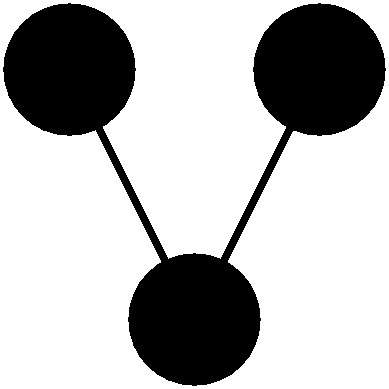
\includegraphics[height=1cm]{./figures/Vmotif.eps} & 
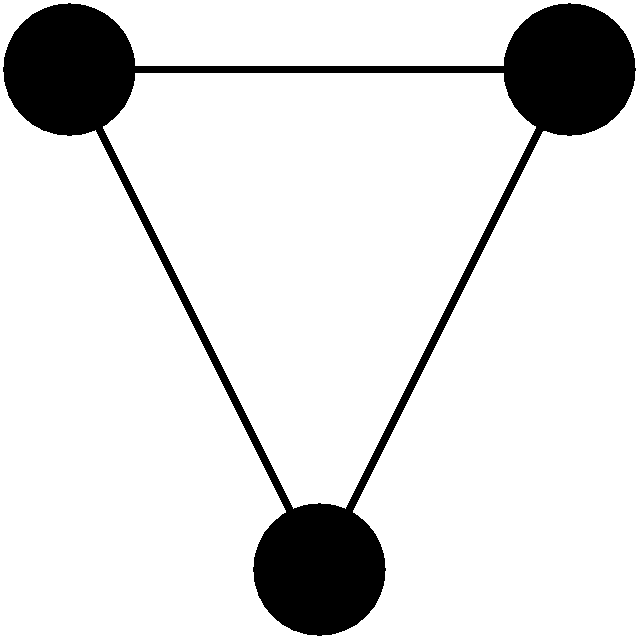
\includegraphics[height=1cm]{./figures/nablamotif.eps} & 
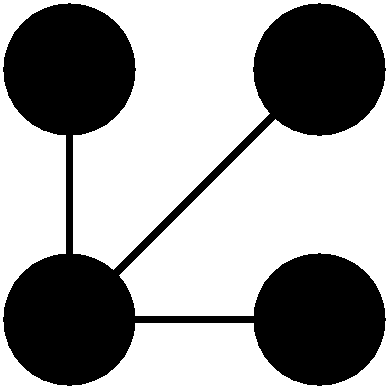
\includegraphics[height=1cm]{./figures/starmotif.eps}  & 
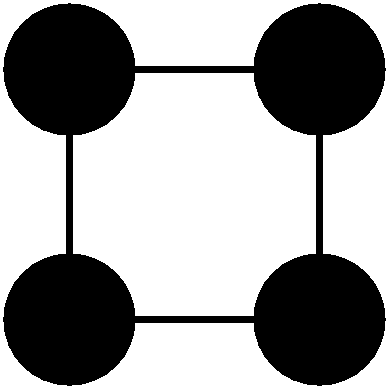
\includegraphics[height=1cm]{./figures/squaremotif.eps}\\
   $\mathsf{V}$ & triangle & 4-star & square \\
   \end{tabular}
 \end{center}

\itemorange We cover a large range for $\Esp N(\mbf)$ (from 0.07 to 1075.5).

\end{itemize}

\end{slide}
}
%----------------------------------------------------

%----------------------------------------------------
\overlays{1}{%
\begin{slide}{Expectedly frequent motif count distribution}

Gaussian (\textcolor{red}{--}), Poisson (--) and
Geometric-Poisson (\textcolor{green}{--})

\includegraphics[width=10cm]{./figures/hist_200_0.005_0.5_0.1_V.eps} 

\vspace{-7.5cm}

\hspace*{5cm}
\includegraphics[width=7cm]{./figures/PPPlot_200_0.005_0.5_0.1_V.eps} 

\end{slide}
}
%----------------------------------------------------


%----------------------------------------------------
\overlays{1}{%
\begin{slide}{Approximation for expectedly frequent motif}

\hspace*{-10mm}
\begin{tabular}{|c|c|}
\hline
{\tiny simulation parameters} &  motif $\Vsf$ \\
\hline
{\tiny
\begin{tabular}{c|c|c|c}
$n$ & $\overline{\pi}$ & $\alpha$ (\%)& $\gamma$ (\%)\\ \hline
200     & 0.5   & 10    & 10   \\
200     & 0.5   & 10    & 90   \\
200     & 0.5   & 50    & 10   \\
200     & 0.5   & 50    & 50   \\
200     & 0.5   & 50    & 90  \\
\end{tabular} 
} 
&
{\tiny
\begin{tabular}{c|c|c|c|c|c|c|c}
$\Esp$ & $\mathbb{V}$ & $\lambda$ & $\frac{1}{1-a}$  & $D_G$ & $D_{GP}$ &
       $\hat{F}_G$ & \org{$\hat{F}_{GP}$} \\ \hline
159.5   & 2034.0        & 23.1 & 6.66   & 20.4 & 19.7 & 2.5 & \org{1.6} \\
104.9   & 590.5         & 31.6 & 3.33   & 15.2 & 14 & 1.9 & \org{1.2}\\
98.5    & 484.0         & 33.3 & 2.27   & 13.1 & 12.6 & 1.1 & \org{0.7}\\
98.5    & 484.0         & 33.2 & 2.27   & 14.3 & 13.2 & 1.6 & \org{1.1}\\
98.5    & 488.4         & 33.1 & 2.27   & 14.5 & 14.8 & 2.5 & \org{0.9}\\
\end{tabular}
}
\\
\hline
\end{tabular}

\vspace{5mm}

Criteria to assess the goodness-of-fit:
\begin{itemize}
\itemorange $D_G$ (resp. $D_{GP}$): \textbf{total variation distance} between the empirical
dist. and the Gaussian (resp. Geometric-Poisson) dist.

\itemorange $\hat{F}_G$ (resp. $\hat{F}_{GP}$): \textbf{empirical proba. of
exceeding the 0.99 quantile} of the Gaussian (resp. Geometric-Poisson) dist.

\end{itemize}

\end{slide}
}
%----------------------------------------------------

%----------------------------------------------------
\overlays{1}{%
\begin{slide}{Expectedly rare motif count distribution}

Gaussian (\textcolor{red}{--}), Poisson (--) and
Geometric-Poisson (\textcolor{green}{--})

\includegraphics[width=10cm]{./figures/hist_200_0.01_0.1_0.1_C.eps} 

\vspace{-7cm}

\hspace*{5cm}
\includegraphics[width=7cm]{./figures/PPPlot_200_0.01_0.1_0.1_C.eps} 
\end{slide}
}
%----------------------------------------------------




%----------------------------------------------------
\overlays{1}{%
\begin{slide}{Approximation for expectedly rare motif}

\vspace{1mm}

\hspace*{-10mm}
\begin{tabular}{|c|c|}
\hline
{\tiny simulation parameters} &  motif $\square$ \\
\hline
{\tiny
\begin{tabular}{c|c|c|c}
$n$ & $\overline{\pi}$ & $\alpha$ (\%)& $\gamma$ (\%)\\ \hline
200&1&10&10   \\
200&1&10&90   \\
200&1&50&10   \\
200&1&50&50   \\
200&1&50&90   \\
\end{tabular} 
} 
&
{\tiny
\begin{tabular}{c|c|c|c|c|c|c|c}
$\Esp$ & $\mathbb{V}$ & $\lambda$ & $\frac{1}{1-a}$  & $D_G$ & $D_{GP}$ &
       $\hat{F}_G$ & \org{$\hat{F}_{GP}$} \\ \hline
7.31&21.72&3.68& 2 &11.8&5.4&3.2&\org{0.9}\\
2.57&3.42&2.21 & 1.16 &9.3&2.7&3.6&\org{0.5}\\
2.74&3.69&2.33 & 1.17 &12.3&3.6&4.7&\org{1.2}\\
1.94&2.40&1.74 & 1.11  &11.3&2.0&3.2&\org{1.6}\\
2.74&3.72&2.32 & 1.17 &10.8&4.5&3.7&\org{0.7}\\
\end{tabular}
}
\\
\hline
\end{tabular}

\vspace{5mm}

{\scriptsize
Criteria to assess the goodness-of-fit:
\begin{itemize}
\itemorange $D_G$ (resp. $D_{GP}$): total variation distance between the empirical
dist. and the Gaussian (resp. Geometric-Poisson) dist.

\itemorange $\hat{F}_G$ (resp. $\hat{F}_{GP}$): empirical proba. of
exceeding the 0.99 quantile of the Gaussian (resp. Geometric-Poisson) dist.

\end{itemize}

}

\end{slide}
}
%----------------------------------------------------




%----------------------------------------------------
\overlays{1}{%
\begin{slide}{Conclusions for the simulation study}

\begin{itemize}
 \itemorange Our analytical expressions for $\Esp N$ and $\Var N$ are correct.

 \itemorange The Poisson approximation is not satisfactory.

\itemorange The Geometric-Poisson approximation outperforms the
Gaussian approximation for both criteria in all cases, especially for
``rare'' motifs.

 \itemorange The 0.99 quantile is underestimated by the Gaussian approximation:  \\
{\bf{$\rightarrow$}} false positive results.

  \itemorange The total variation distance is high
    for both approximations in some cases, especially for frequent and
    highly self overlapping motifs.

  \itemorange The clumps size distribution is not geometric $\ldots$
\end{itemize}
\end{slide}
}
%----------------------------------------------------

%----------------------------------------------------
\overlays{1}{%
\begin{slide}{Application to the {\it H. pylori} PPI network}
\begin{itemize}
\itemorange Protein-protein interaction network: 706 proteins (nodes)
and 1420 interactions (edges).

 \itemorange ERMG was fitted to the network and 4 groups of
 connectivity were selected using a model selection criterion.
 
\itemorange Goodness-of-fit for the degree distribution (PP-plot):
 \end{itemize}

\vspace{-5mm}

\begin{center}
\includegraphics[width=4cm]{./figures/hist-deg-HPylo.eps}   
\end{center}
\end{slide}
}
%----------------------------------------------------

%----------------------------------------------------
\overlays{1}{%
\begin{slide}{Exceptional motifs of size 3 and 4}

\begin{center}
\begin{tabular}{c|r|rr|c} 
    Motif & $N_{\text{obs}}$ & $\mathbb{E}_{\text{ermg}} N$ 
    & $\sigma_{\text{ermg}}(N)$ & $\prob(\mathcal{GP}\geq N_{\text{obs}})$\\
    \hline
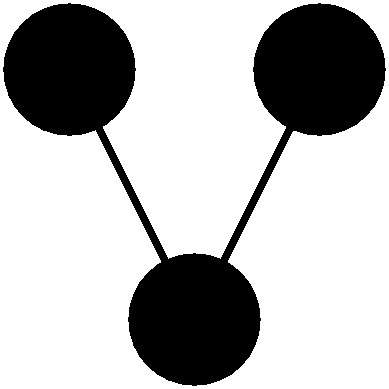
\includegraphics[width=0.5cm]{./figures/Vmotif.eps}             &  13888        & 13118       & 2599      & 3.66\,10$\mathbf{^{-1}}$\\
\includegraphics[width=0.5cm]{./figures/triangle.eps}      &  75           & 64.4       & 20.0            & 2.87\,10$\mathbf{^{-1}}$    \\
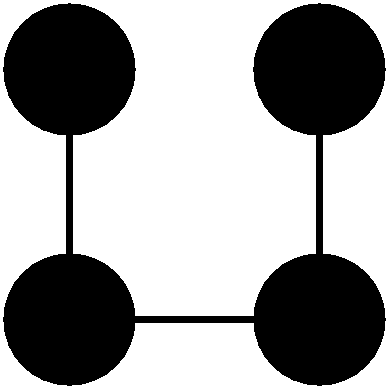
\includegraphics[width=0.5cm]{./figures/chainmotif.eps}         &  87869        & 90059       & 26064      & 5.04\,10$\mathbf{^{-1}}$\\
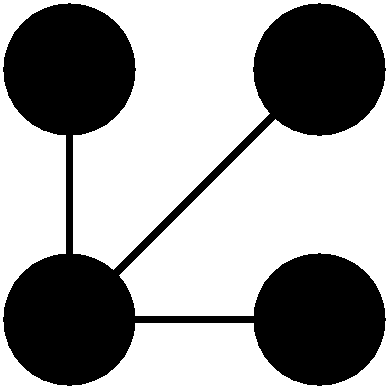
\includegraphics[width=0.5cm]{./figures/starmotif.eps}          &  109113       & 89372       & 26423      & 2.17\,10$\mathbf{^{-1}}$\\
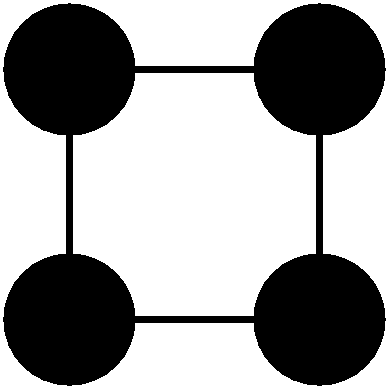
\includegraphics[width=0.5cm]{./figures/squaremotif.eps}        &  979          & 492        & 202      & 1.86\,10$\mathbf{^{-1}}$\\
\includegraphics[width=0.5cm]{./figures/whisk.eps}            &  3219         & 2756       & 1087      & 3.06\,10$\mathbf{^{-1}}$ \\
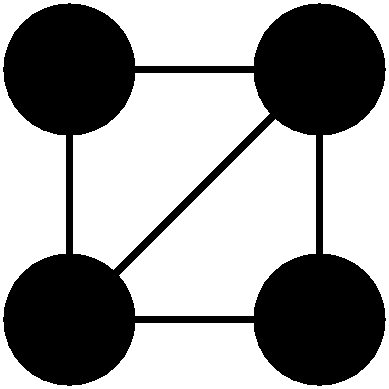
\includegraphics[width=0.5cm]{./figures/halfclique.eps}         &  79           & 33.2       & 19.5      & \textcolor{magenta}{2.56\,10$\mathbf{^{-2}}$}       \\
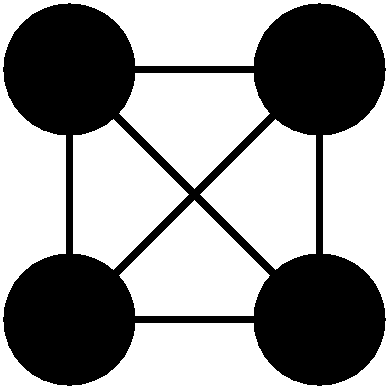
\includegraphics[width=0.5cm]{./figures/clique.eps}             &  0            & 0.165      & 0.432      & 1    
  \end{tabular}
\end{center}

\end{slide}
}


%----------------------------------------------------

%----------------------------------------------------
\overlays{1}{%
\begin{slide}{Comparison with the Mfinder software}

\centerline{{\tt \org{Mfinder: www.weizmann.ac.il/mcb/UriAlon/}}}

\vspace{5mm}

{\scriptsize

\hspace*{-5mm}
\begin{tabular}{c|r|rr|rrr|c} 
  Motif & $N_{\text{obs}}$ & $\mathbb{E}_{\text{ermg}} N$ & $\sigma_{\text{ermg}}(N)$ 
&$\overline{N}_{100}$&$\overline{\sigma }_{100}$&Z-score & tail $\Ncal(0,1)$ \\
    \hline
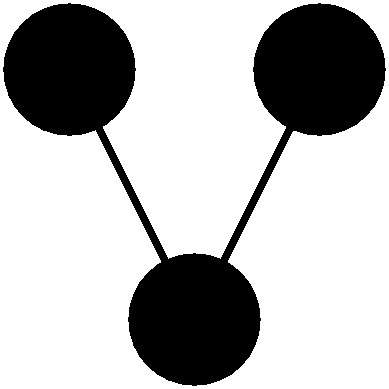
\includegraphics[width=0.5cm]{./figures/Vmotif.eps}     &  13888 &13118  & 2599
& \org{13648} & \org{51.8} & \org{4.63} & \rose{1.82\,10$\mathbf{^{-6}}$}    \\
\includegraphics[width=0.5cm]{./figures/triangle.eps}   &  75    &64.4   & 20.0
& \org{155}   & \org{17.3} & \org{-4.63}& \rose{1.82\,10$\mathbf{^{-6}}$}     \\
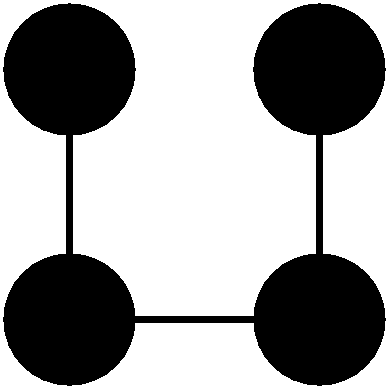
\includegraphics[width=0.5cm]{./figures/chainmotif.eps} &  87869  &90059 & 26064
& \org{112532} & \org{1957} & \org{-12.60}& \rose{1.05\,10$\mathbf{^{-36}}$}  \\
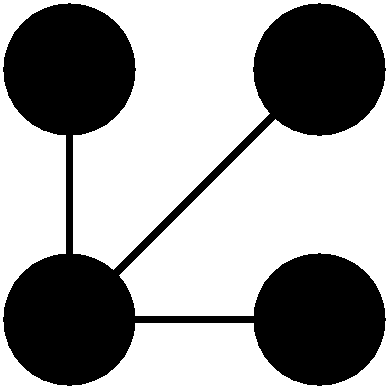
\includegraphics[width=0.5cm]{./figures/starmotif.eps}  &  109113 & 89372  & 26423
& \org{103186} & \org{1084} & \org{5.47}& \rose{2.27\,10$\mathbf{^{-8}}$}     \\
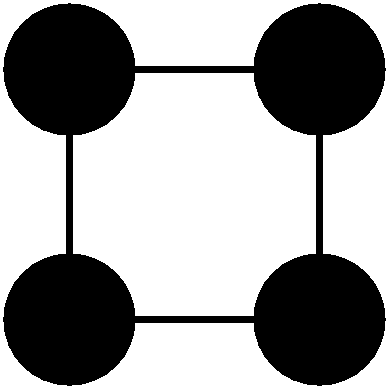
\includegraphics[width=0.5cm]{./figures/squaremotif.eps}&  979    & 492   & 202
& \org{796} & \org{64.7} & \org{2.84}& \rose{2.25\,10$\mathbf{^{-3}}$}    \\
\includegraphics[width=0.5cm]{./figures/whisk.eps}      &  3219   & 2756  & 1087
& \org{8734} & \org{945} & \org{-5.84}& \rose{2.61\,10$\mathbf{^{-9}}$}   \\
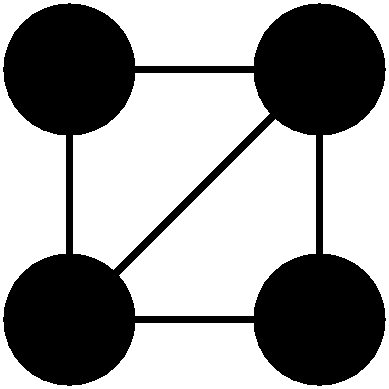
\includegraphics[width=0.5cm]{./figures/halfclique.eps} &  79     & 33.2  & 19.5
& \org{273} & \org{66.7}& \org{-2.90}& \rose{1.85\,10$\mathbf{^{-3}}$}    \\
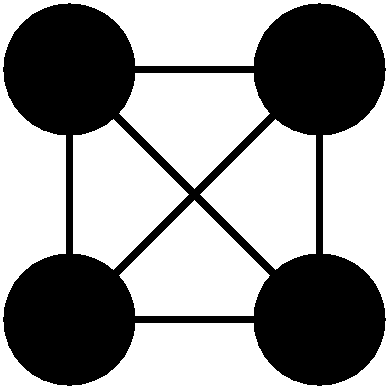
\includegraphics[width=0.5cm]{./figures/clique.eps}     &  0      & 0.165 & 0.432
& \org{6.2} & \org{3.7} & \org{-1.70}& \rose{4.45\,10$\mathbf{^{-2}}$}       
  \end{tabular}
}

\end{slide}
}


%----------------------------------------------------



%----------------------------------------------------
\overlays{1}{%
\begin{slide}{Conclusions \& future directions }
\begin{itemize}
 \itemorange We proposed a statistical method to assess the exceptionality of network motifs.
 
\itemorange The method to calculate the moments of the count is
general and can be applied to any random graph model with stationary
distribution.

 \itemorange The Geometric-Poisson approximation for the count
 distribution works well (better than the Gaussian) on simulated data. 

 \end{itemize}

Directions: 

\begin{itemize}
 \itemblue Distribution of the clump size. 

\itemblue Exceptionality of colored motifs.
\end{itemize}
\end{slide}
}
%----------------------------------------------------

  
%----------------------------------------------------
\overlays{1}{%
\begin{slide}{ERMG: estimation procedure}

\begin{itemize}
\itemorange The aim is to maximize the log-likelihood $\Lcal(\Xbf)$,

\itemorange $\ldots$ but $\Lcal(\Xbf)$ is not calculable because of hidden
groups ($\Zbf$, $Z_i$ is the group of node $i$).

\itemorange EM algorithm is classical to fit mixture models,

\itemorange $\ldots$ but cannot be used because $\prob(\Zbf\:|\:\Xbf)$ is not
computable (all vertices are potentially connected, no local
dependence)

\itemblue Strategy = \textbf{variational approach}
\begin{itemize}
\itemblue maximization of
$\Lcal(\Xbf)-KL(\prob(\Zbf\:|\:\Xbf),Q_R(\Zbf))$ where $Q_R$ is the
best approximation of $\prob(\Zbf\:|\:\Xbf)$ within a class of 'nice'
distributions. $\Rightarrow$ estimator of $\prob(Z_i=q|\Xbf)$.
\itemblue analytical expressions for $\widehat{\alpha}_q$ and
$\widehat{\pi}_{q,\ell}$
\itemblue iterative algorithm
\end{itemize}
\end{itemize}

\end{slide}
}
%----------------------------------------------------

  
%----------------------------------------------------
\overlays{1}{%
\begin{slide}{ERMG: model selection procedure}

\begin{itemize}
\itemorange Heuristic penalized likelihood criterion inspired from BIC (ICL)

\itemblue The completed log-likelihood $\Lcal(\Xbf, {\Zbf})$  
is the sum 
{\scriptsize
\begin{tabular}{p{3.5cm}cp{6cm}}
$\displaystyle{\sum_i \sum_q \ind\{Z_i=q\} \log \alpha_q}$
&+&
$\displaystyle{\sum_{i,j>i} \sum_{q,\ell}
  \ind\{Z_i=q\}\ind\{Z_j=\ell\}\log b(X_{ij};\pi_{q,\ell})}$\\
&&\\
$(Q-1)$ independent proportions $\alpha_q$'s and
  $n$ terms
&&
$Q(Q+1)/2$ probabilities $\pi_{q,\ell}$'s and \qquad$n(n-1)/2$ terms
\end{tabular}
}

\itemblue The heuristic criterion is then:
$$
- 2\widehat{\Lcal}(\Xbf, \Zbf) + (Q-1) \log n + \frac{Q(Q+1)}2
\log\left[\frac{n(n-1)}2\right].
$$
\end{itemize}


\end{slide}
}
%----------------------------------------------------

%----------------------------------------------------
\overlays{1}{%
\begin{slide}{Illustration of ERMG}

The ERMG has been adjusted to
\begin{itemize}
\itemorange \textit{E. coli} reaction network: 605 vertices, 1782
edges.\\
(data curated by V. Lacroix and M.-F. Sagot).

\itemorange $Q=21$ groups selected 

\begin{center}
Group proportions $\widehat{\alpha}_q$ (\%). \\
\epsfig{file = figures/Ecoli-Complet-ERMG-Ward-Q21_param.eps,
      height=3cm, width=6cm, clip=, bbllx=75, bblly=570, bburx=530,
      bbury=770}   
\end{center}

\itemorange Many small groups correspond to cliques or
    pseudo-cliques. 
\end{itemize}


\end{slide}
}
%----------------------------------------------------

    
%----------------------------------------------------
\overlays{1}{%
\begin{slide}{Dot plot representation of the network}

\begin{center}
   \epsfig{file = figures/Ecoli-Complet-ERMG-Ward-Q21_class.eps,
      height=8cm, width=8cm, clip=,bbllx=70, bblly=440, bburx=540,
      bbury=770} 
\end{center}


\end{slide}
}
%----------------------------------------------------

%----------------------------------------------------
\overlays{1}{%
\begin{slide}{Dot plot representation (zoom)}
{\scriptsize
\vspace*{-4mm}

\begin{tabular}{lc}
  \begin{tabular}{p{3.5cm}}
    Sub-matrix of $\pi$:\\ \\
    \begin{tabular}{c|ccc}
      $q, \ell$ & 1 & 10 & 16 \\
      \hline 
      1 & \org{1.0}&& \\ 
       10 & {\sl .43}  & .67&  \\ 
      16 & \org{1.0} &{\sl 0} & \org{1.0} \\
    \end{tabular}
   \\ 
  \end{tabular}
  &
 \begin{tabular}{l}
    \hspace{0.55cm}
    \epsfig{file = figures/Ecoli-Complet-ERMG-Ward-Q21_class.eps,
      height=5.5cm, width=5.5cm, clip=,bbllx=90, bblly=485, bburx=277,
      bbury=605.5}   
  \end{tabular}  \\
  \vspace{-6mm}

%   \\ \\ \\
   \begin{tabular}{p{3.5cm}}
    {Vertex degrees $K_i$'s.}  \\  
    Mean degree in the last group: 
    $\overline{K}_{21} = 2.6$ \\ 
  \end{tabular}
  &
\vspace{-1cm}
 
  \begin{tabular}{l}
    \epsfig{file = figures/Ecoli-Complet-ERMG-Ward-Q21_class.eps,
    width=6.1cm, height=2.5cm, clip=, bbllx=70, bblly=105, bburx=277,
    bbury=245}   
  \end{tabular}
\end{tabular}
}
\end{slide}
}
%----------------------------------------------------
  
%----------------------------------------------------
\overlays{1}{%
\begin{slide}{Model fit}

\begin{itemize}
\itemorange \textbf{Degrees}: Poisson mixture versus empirical
distribution\\
 \hspace*{7.5cm}PP-plot
\begin{center}
\includegraphics[height=4cm,width=10cm]{./figures/Ecoli-Complet-ERMG-Ward-Q21_degree.eps}
\end{center}
\itemorange\textbf{Clustering coefficient}:\\
\begin{center}
\begin{tabular}{ccc}
  Empirical & ERMG ($Q = 21$) & ER ($Q = 1$)\\
  \hline
  0.626 & 0.544 & 0.0098
\end{tabular}
\end{center}

\end{itemize}


\end{slide}
}
%----------------------------------------------------

\end{document}
